Before we proceed to the data processing, let us first give a brief introduction
to the data set that we consider, which is the Google cluster-usage traces
\cite{reiss2011}. The traces were collected over 29 days in May 2011 and
encompass more than 12 thousand machines serving requests from more than 900
users.

In the data set's parlance, a user request is a job, and a job comprises one or
several tasks, and a task is a Linux program to be run on a single machine.
Apart from other data, the data set contains the so-called resource-usage table.
The table keeps track of the resource usage of the tasks with the sampling
interval of five minutes. Specifically, the average and maximum values of the
CPU, memory, and disk usage are provided. Each record corresponds to a
particular task over a particular five-minute interval, and there are more than
1.2 billion records corresponding to more than 24 million tasks.

The resource-usage table of the tasks is provided in the form of 500 archives.
Each archive contains a single \up{CSV} file, which, in turn, contains
performance measurements over a certain time window. Such a format is rather in
convenient given the way the data are supposed to be queried at the learning
stage. For instance, in order to find all the data points that belong to a
particular task, one has to search, in principle, in all the archives. Such a
querying strategy is not practical as reading data is a core operation, which
has to be undertaken millions of times during a learning session. The situation
is exacerbated even further when multiple learning sessions are to be performed,
which is the most common scenario in practice. All in all, an efficient
data-processing pipeline is needed, which is what we shall develop in this
section.

\subsection{Grouping}
The \up{CSV} data from the 500 archives are distributed into separate \up{CSV}
files so that each such file contains all the data points that belong to a
particular job. As a result, there are as many \up{CSV} files as there are jobs.

\subsection{Indexing}
She sells seashells on the seashore.

\subsection{Selection}
\begin{figure}[t]
  \centering
  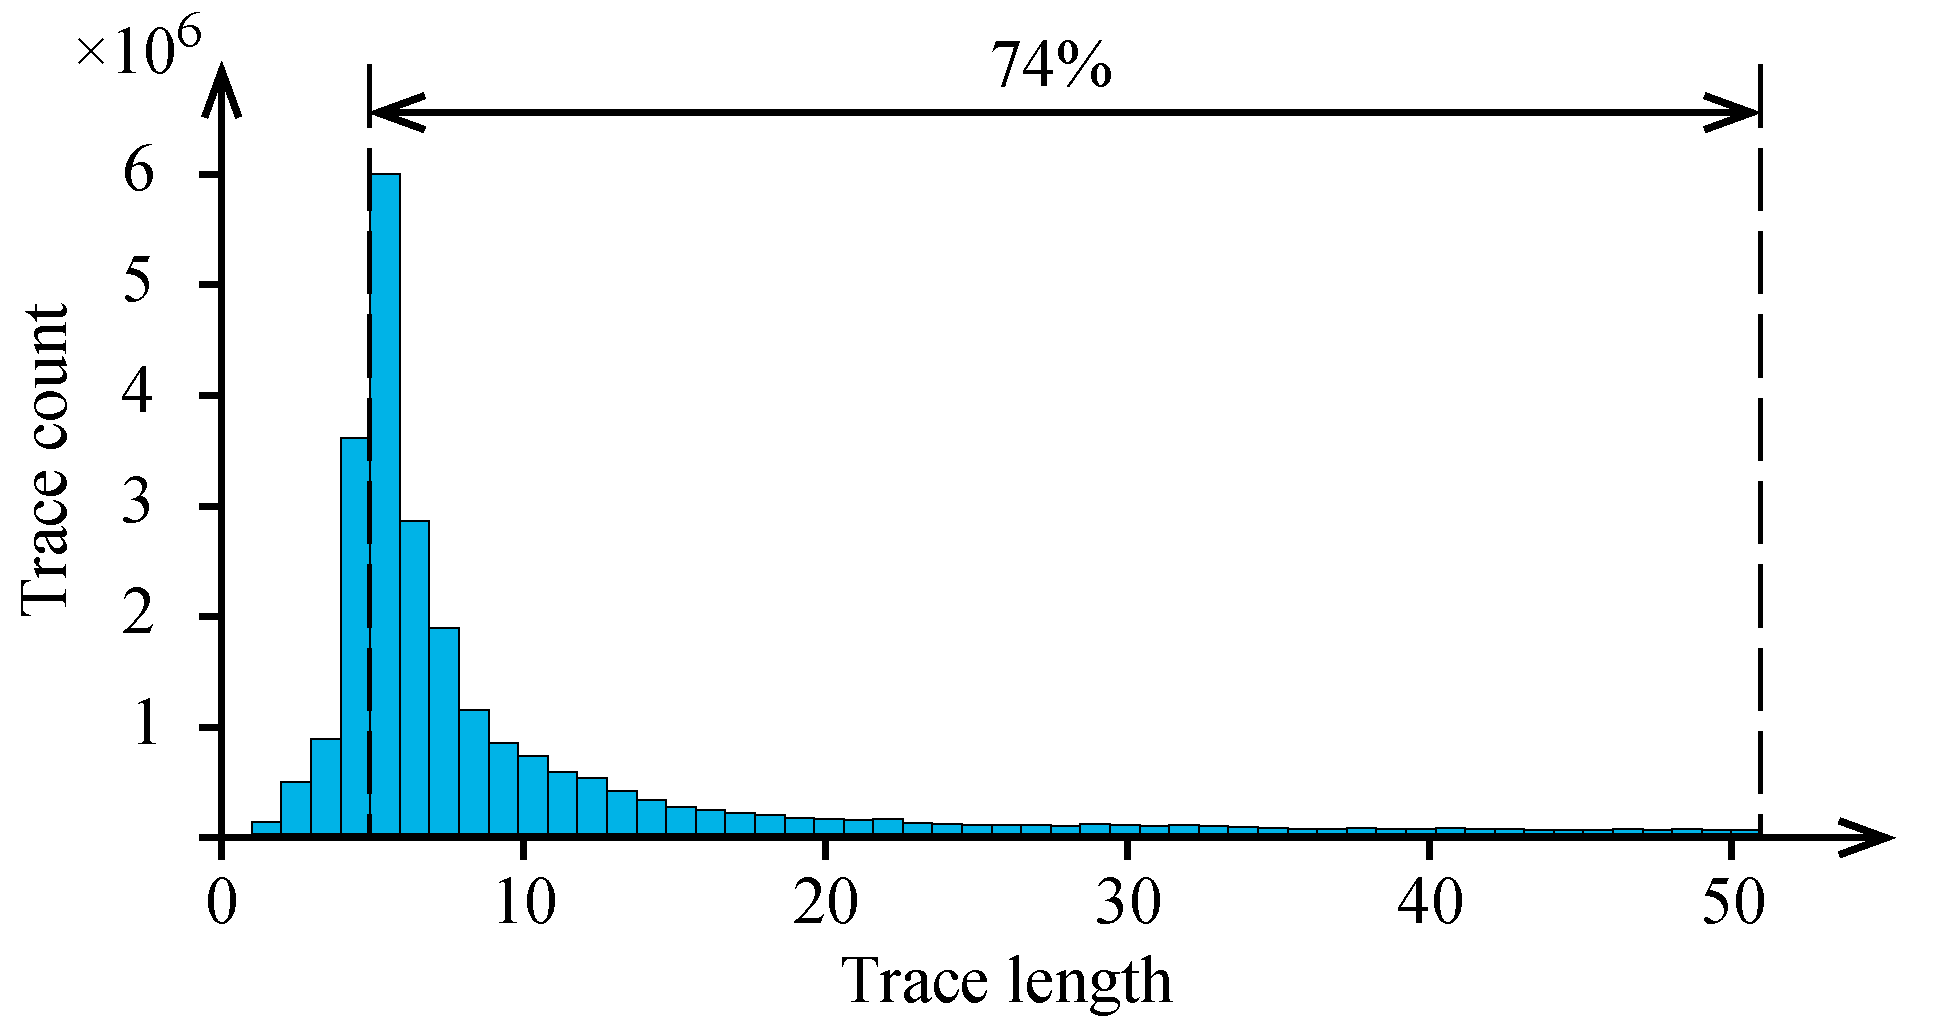
\includegraphics[width=1.0\columnwidth]{include/assets/figures/histogram.pdf}
  \caption{The histogram of the lengths of the resource-usage traces.}
  \flab{histogram}
\end{figure}

The histogram of the resource-usage traces' lengths can be seen in
\fref{histogram}; the histogram has been truncated on the right-hand side in
order to show the bulk of the distribution better. In our experiments, we
consider only those traces that contain 5--50 data points, which constitute
around 74\% of the total number of traces. The upper bound discards a negligibly
small portion of the data while the lower one ensures that there is a sufficient
number of data points for experimentation.
